\documentclass[9pt,a4paper,twocolumn]{article}
\usepackage[a4paper,top=19mm,bottom=18mm,left=19mm,right=19mm,columnsep=6mm]{geometry}
\usepackage{mathptmx}
\usepackage[T1]{fontenc}
\usepackage{xcolor,graphicx,booktabs,tabularx,hyperref,fancyhdr}
\definecolor{journalblue}{HTML}{004A93}
\definecolor{headingblue}{HTML}{0070C0}
\definecolor{rulegreen}{HTML}{557030}
\definecolor{abstractgreen}{HTML}{F1F5E8}
\hypersetup{colorlinks=true,urlcolor=journalblue,linkcolor=journalblue}
\pagestyle{fancy}\fancyhf{}
\fancyhead[R]{\scriptsize Maddipatla Naga Venkata Sai Krishna \& Asit Kumar Sahoo, Sch J Eng Tech}
\renewcommand{\headrulewidth}{0.5pt}\renewcommand{\headrule}{\hbox to\headwidth{\color{rulegreen}\leaders\hrule height \headrulewidth\hfill}}
\fancyfoot[L]{\scriptsize PLaND $\mid$ Preprint - arXiv identifier pending}
\fancyfoot[R]{\scriptsize\thepage}
\renewcommand{\footrulewidth}{0.5pt}
\setlength{\parindent}{1.2em}\setlength{\parskip}{0.15em}
\makeatletter
\renewcommand\section{\@startsection{section}{1}{0pt}{0.7ex}{0.25ex}{\color{headingblue}\normalfont\large}}
\renewcommand\subsection{\@startsection{subsection}{2}{0pt}{0.6ex}{0.2ex}{\normalfont\normalsize}}
\makeatother
\begin{document}
\twocolumn[
\begin{minipage}{\textwidth}
{\color{journalblue}\LARGE Scholars Journal of Engineering and Technology\par}
\vspace{0.5mm}
{\scriptsize Abbreviated Key Title: Sch J Eng Tech \quad Journal homepage: \url{https://saspublishers.com/journal/sjet/home}\par}
\vspace{2mm}
{\color{rulegreen}\hrule}\vspace{3mm}
{\color{journalblue}\LARGE PLaND - Path to Least Non Determinism\par}
\vspace{1mm}
{\normalsize Maddipatla Naga Venkata Sai Krishna \quad Asit Kumar Sahoo\par}
\vspace{1mm}
{\color{red}\hrule}\vspace{2mm}
\begin{center}\begin{minipage}{0.98\textwidth}\colorbox{journalblue}{\parbox{0.97\textwidth}{\color{white}\textbf{Abstract}\hfill Original Research Article}}
\colorbox{abstractgreen}{\parbox{0.97\textwidth}{Language-model agents often repeat mechanical work because an entire standard operating procedure (SOP) is expressed in natural language. We present Path to Least Non Determinism (PLaND), an evaluation-driven methodology that retains language-model judgment where needed while moving stable steps into references, Python, or Bash. Before measurement, PLaND freezes the model, prompt, harness, data, scorer, seed, runtime settings, permissions, and acceptance rule; only the workflow skill package may evolve. Three new paired replications on a balanced top-10, single-label LEDGAR test subset produced 93.7\% natural-language (NL) and 92.9\% hybrid accuracy in every run. The hybrid passed every absolute viability, non-inferiority, and efficiency gate, reduced mean tokens 40.02\% (376,090 to 225,575.33), and bypassed 411 of 1,000 model calls. Both variants produced identical labels across the three seeds, so observed cross-run disagreement was zero; this floor does not show hybrid-specific variance reduction. CFPB and SpamAssassin repeated their rejection outcomes in all three runs despite token savings. Three document-image workflows remained single-baseline feasibility failures. PLaND therefore supports selective, evidence-bound determinisation rather than unconditional conversion to code.\\[1mm]\textbf{Keywords:} agent skills, deterministic workflows, language-model agents, evaluation, token efficiency, workflow optimization}}
\end{minipage}\end{center}\vspace{2mm}
\end{minipage}
]
\section{Introduction}
Language-model agents are valuable when a task requires interpretation, contextual judgment, or exception handling. They are less valuable when repeatedly asked to parse fixed fields, count items, normalize values, validate a schema, or apply an exact rule. Reusable agent instructions are increasingly packaged as skills: the Agent Skills specification requires \texttt{SKILL.md} and permits references, scripts, and assets [1]; DeepAgents supports open-ended skill use [2]; and LangGraph represents stable workflows as explicit graphs [3]. These systems do not determine which SOP steps should retain model judgment.

PLaND asks: what is the least non-deterministic form of a workflow that still satisfies its measured quality contract? Natural language remains appropriate for ambiguous decisions. Ordinary code is usually preferable for bounded, testable computation. The intended endpoint may therefore be an open-ended agent, a hybrid skill, or a mostly deterministic graph.

The same task makes this progression concrete. Figure 1 reproduces representative numbered lines from the repository's actual LEDGAR skills. The natural-language SOP asks the model to read the complete clause, identify its legal function, compare it with the allowed labels, and select the best label. The hybrid SOP inserts one command step, \texttt{python classify.py}, before those semantic instructions; it accepts only a high-confidence result and otherwise returns to the natural-language steps. A mature graph-based SOP would make stable operations explicit deterministic nodes while retaining model reasoning in only the few nodes that resolve ambiguous clauses. This graph is the preferred mature form when each substitution passes the quality contract; PLaND does not force a workflow to reach it.

\begin{figure*}[t]
\centering
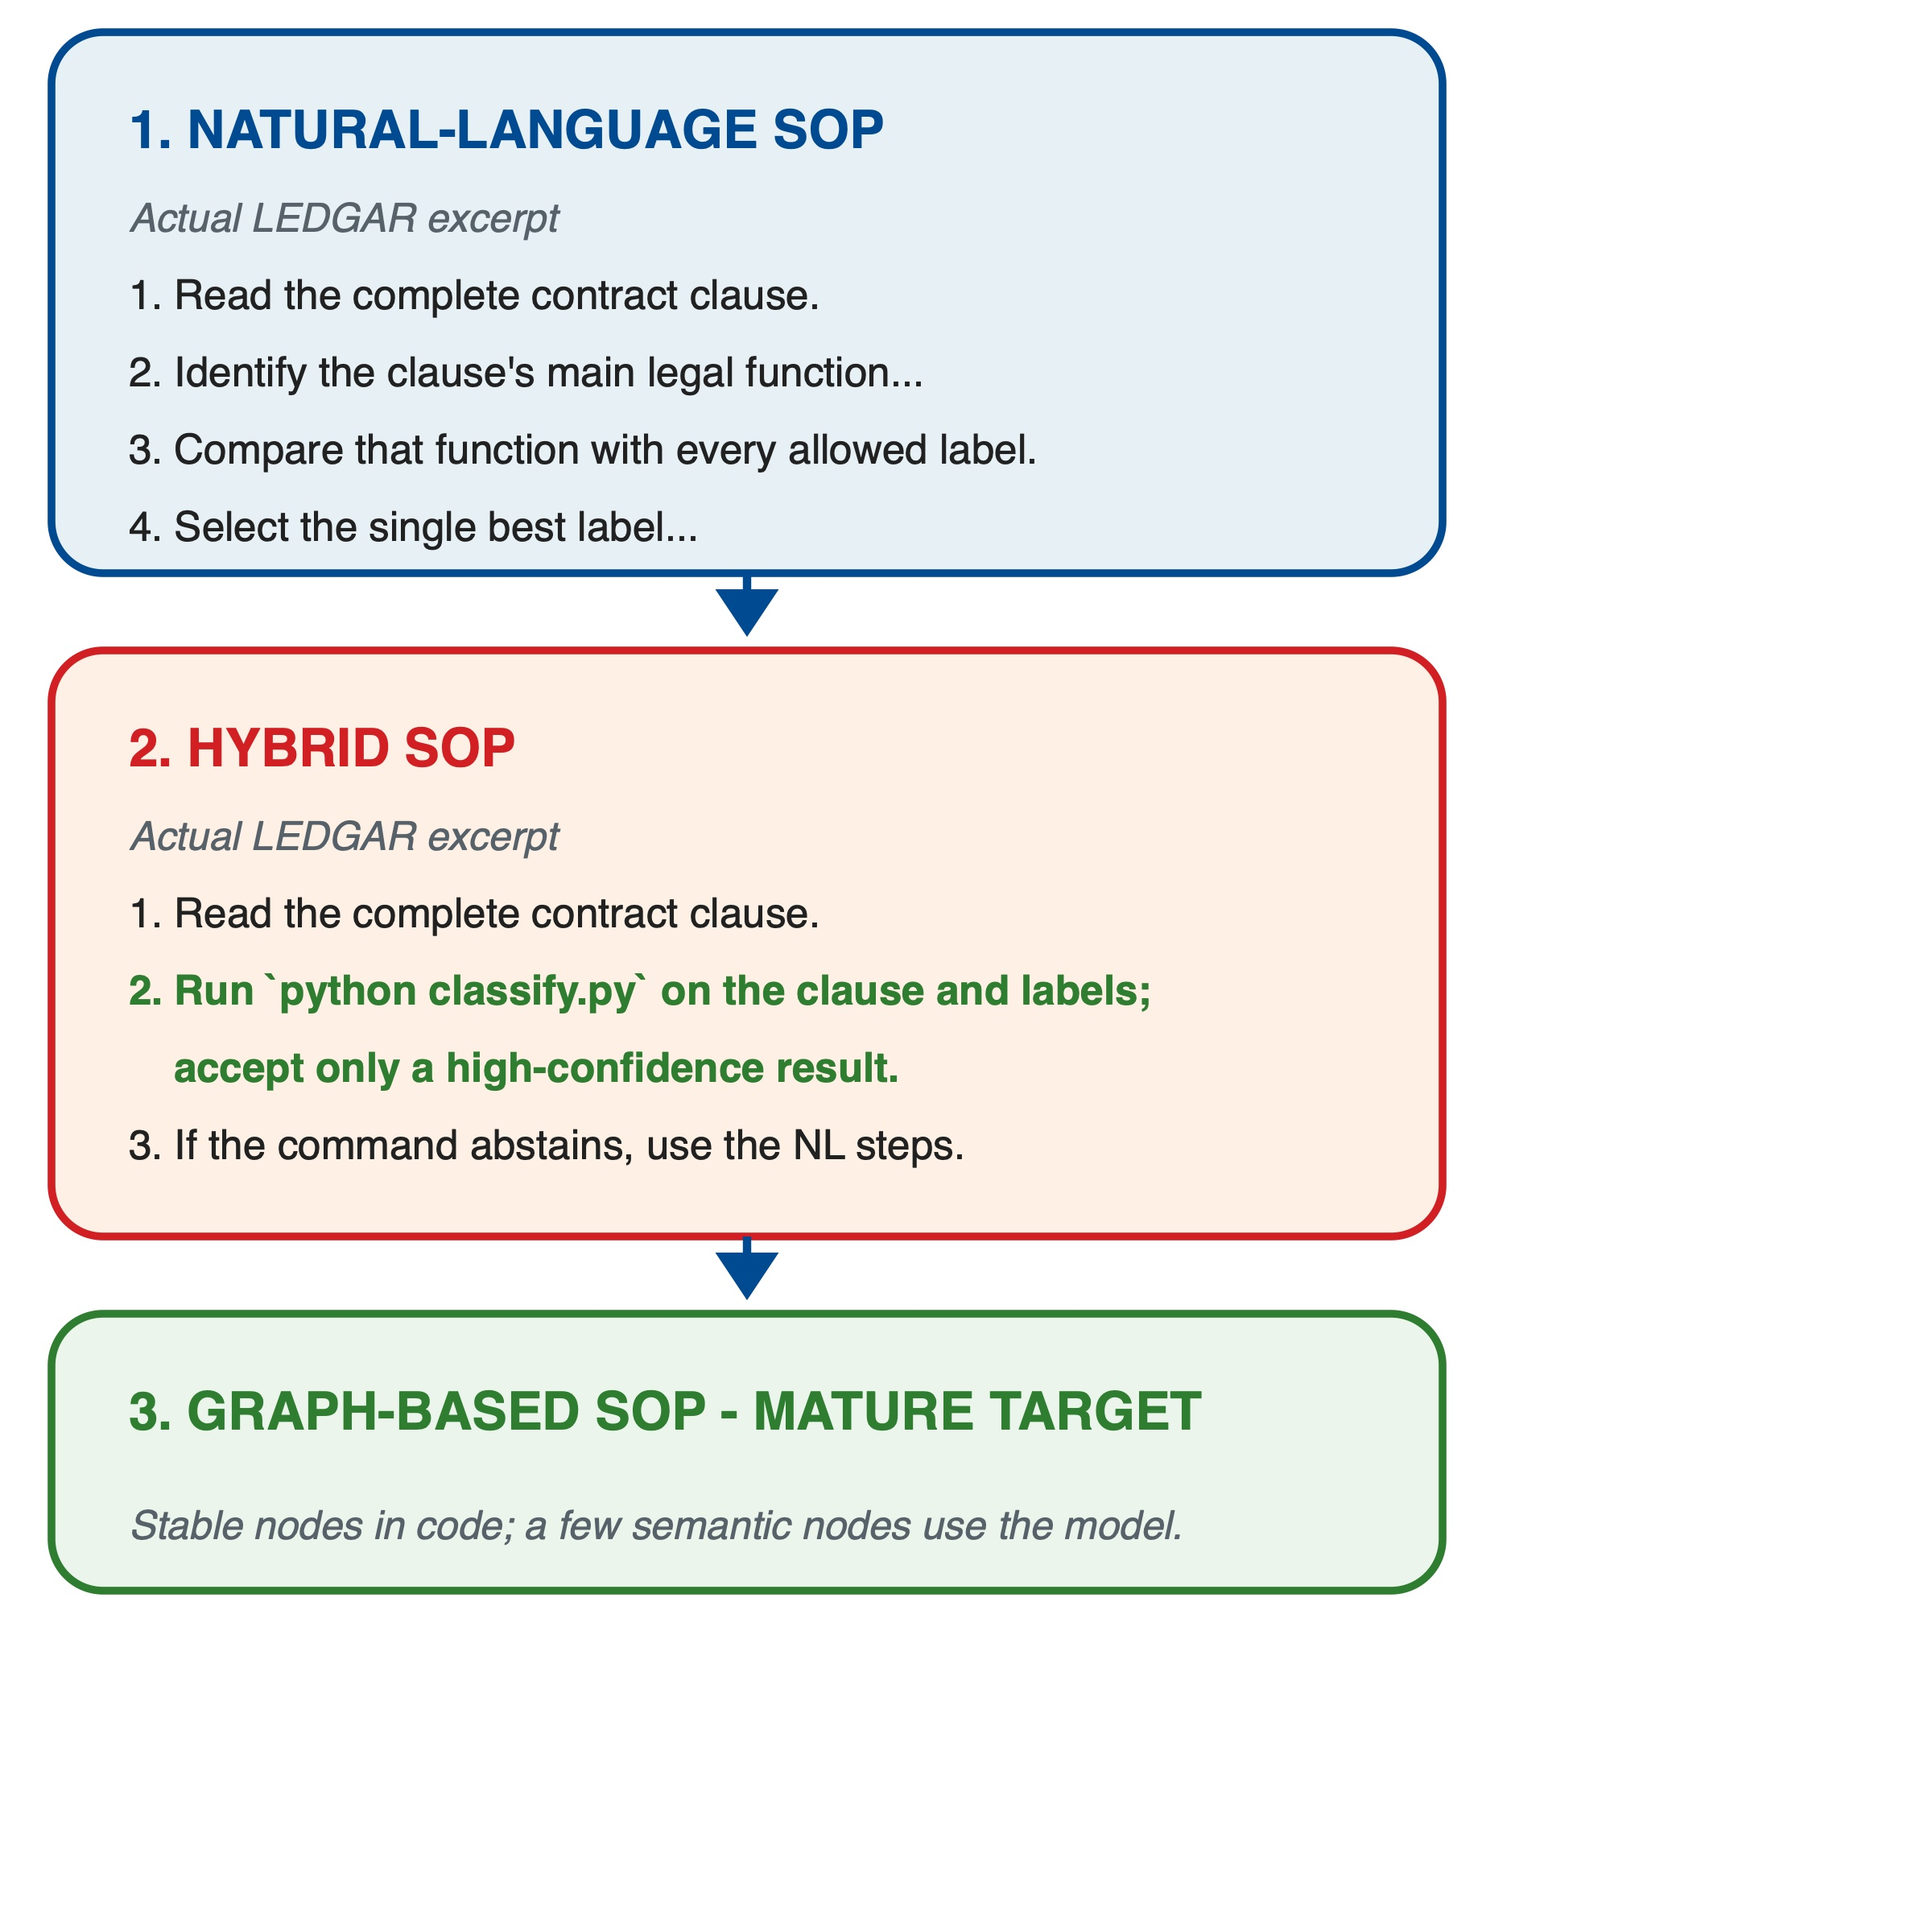
\includegraphics[width=0.64\textwidth]{evolution-path.jpg}
\caption{Actual LEDGAR SOP excerpts and the intended mature endpoint. The natural-language skill contains only English steps. The hybrid skill inserts \texttt{python classify.py}, accepts only a high-confidence result, and uses the English steps when the command abstains. When further validated substitutions are available, the preferred mature endpoint is a graph-based SOP in which stable nodes are deterministic and only a few semantic nodes remain non-deterministic.}
\end{figure*}

Related systems optimize language-model programs, prompts, workflows, or skills. DSPy compiles declarative model pipelines against metrics [4]; AutoFlow and AFlow generate and optimize workflows [5, 6]; and Automated Design of Agentic Systems searches agent designs [7]. SkillOpt, SkillRevise, SkillReducer, and ACES optimize or evaluate reusable skills [8-11]. PLaND contributes a narrower representation path - English instruction, reference, or command - plus a frozen mutation boundary, paired evaluation, explicit rejection records, and a held-out release gate.

We ask whether a hybrid SOP can reduce model-mediated work while remaining inside a fixed quality margin, whether validation gates block efficient but unsafe candidates, whether savings arise from fewer calls rather than prompt shortening alone, and how stable case-level predictions are across a small set of controlled replications.

\section{Material and Methods}
\subsection{Methodology and mutation boundary}
PLaND uses two open-ended skills. \texttt{generate-initial-version} converts natural-language task requirements, approved data sources, and evaluation examples into an initial agent, system prompt, and natural-language SOP. \texttt{pland-evolver} uses development traces to propose bounded changes. Task-local runners and scorers define the executable interface and primary quality measure, so the methodology is not restricted to classification or a particular output type.

\begin{figure*}[t]
\centering
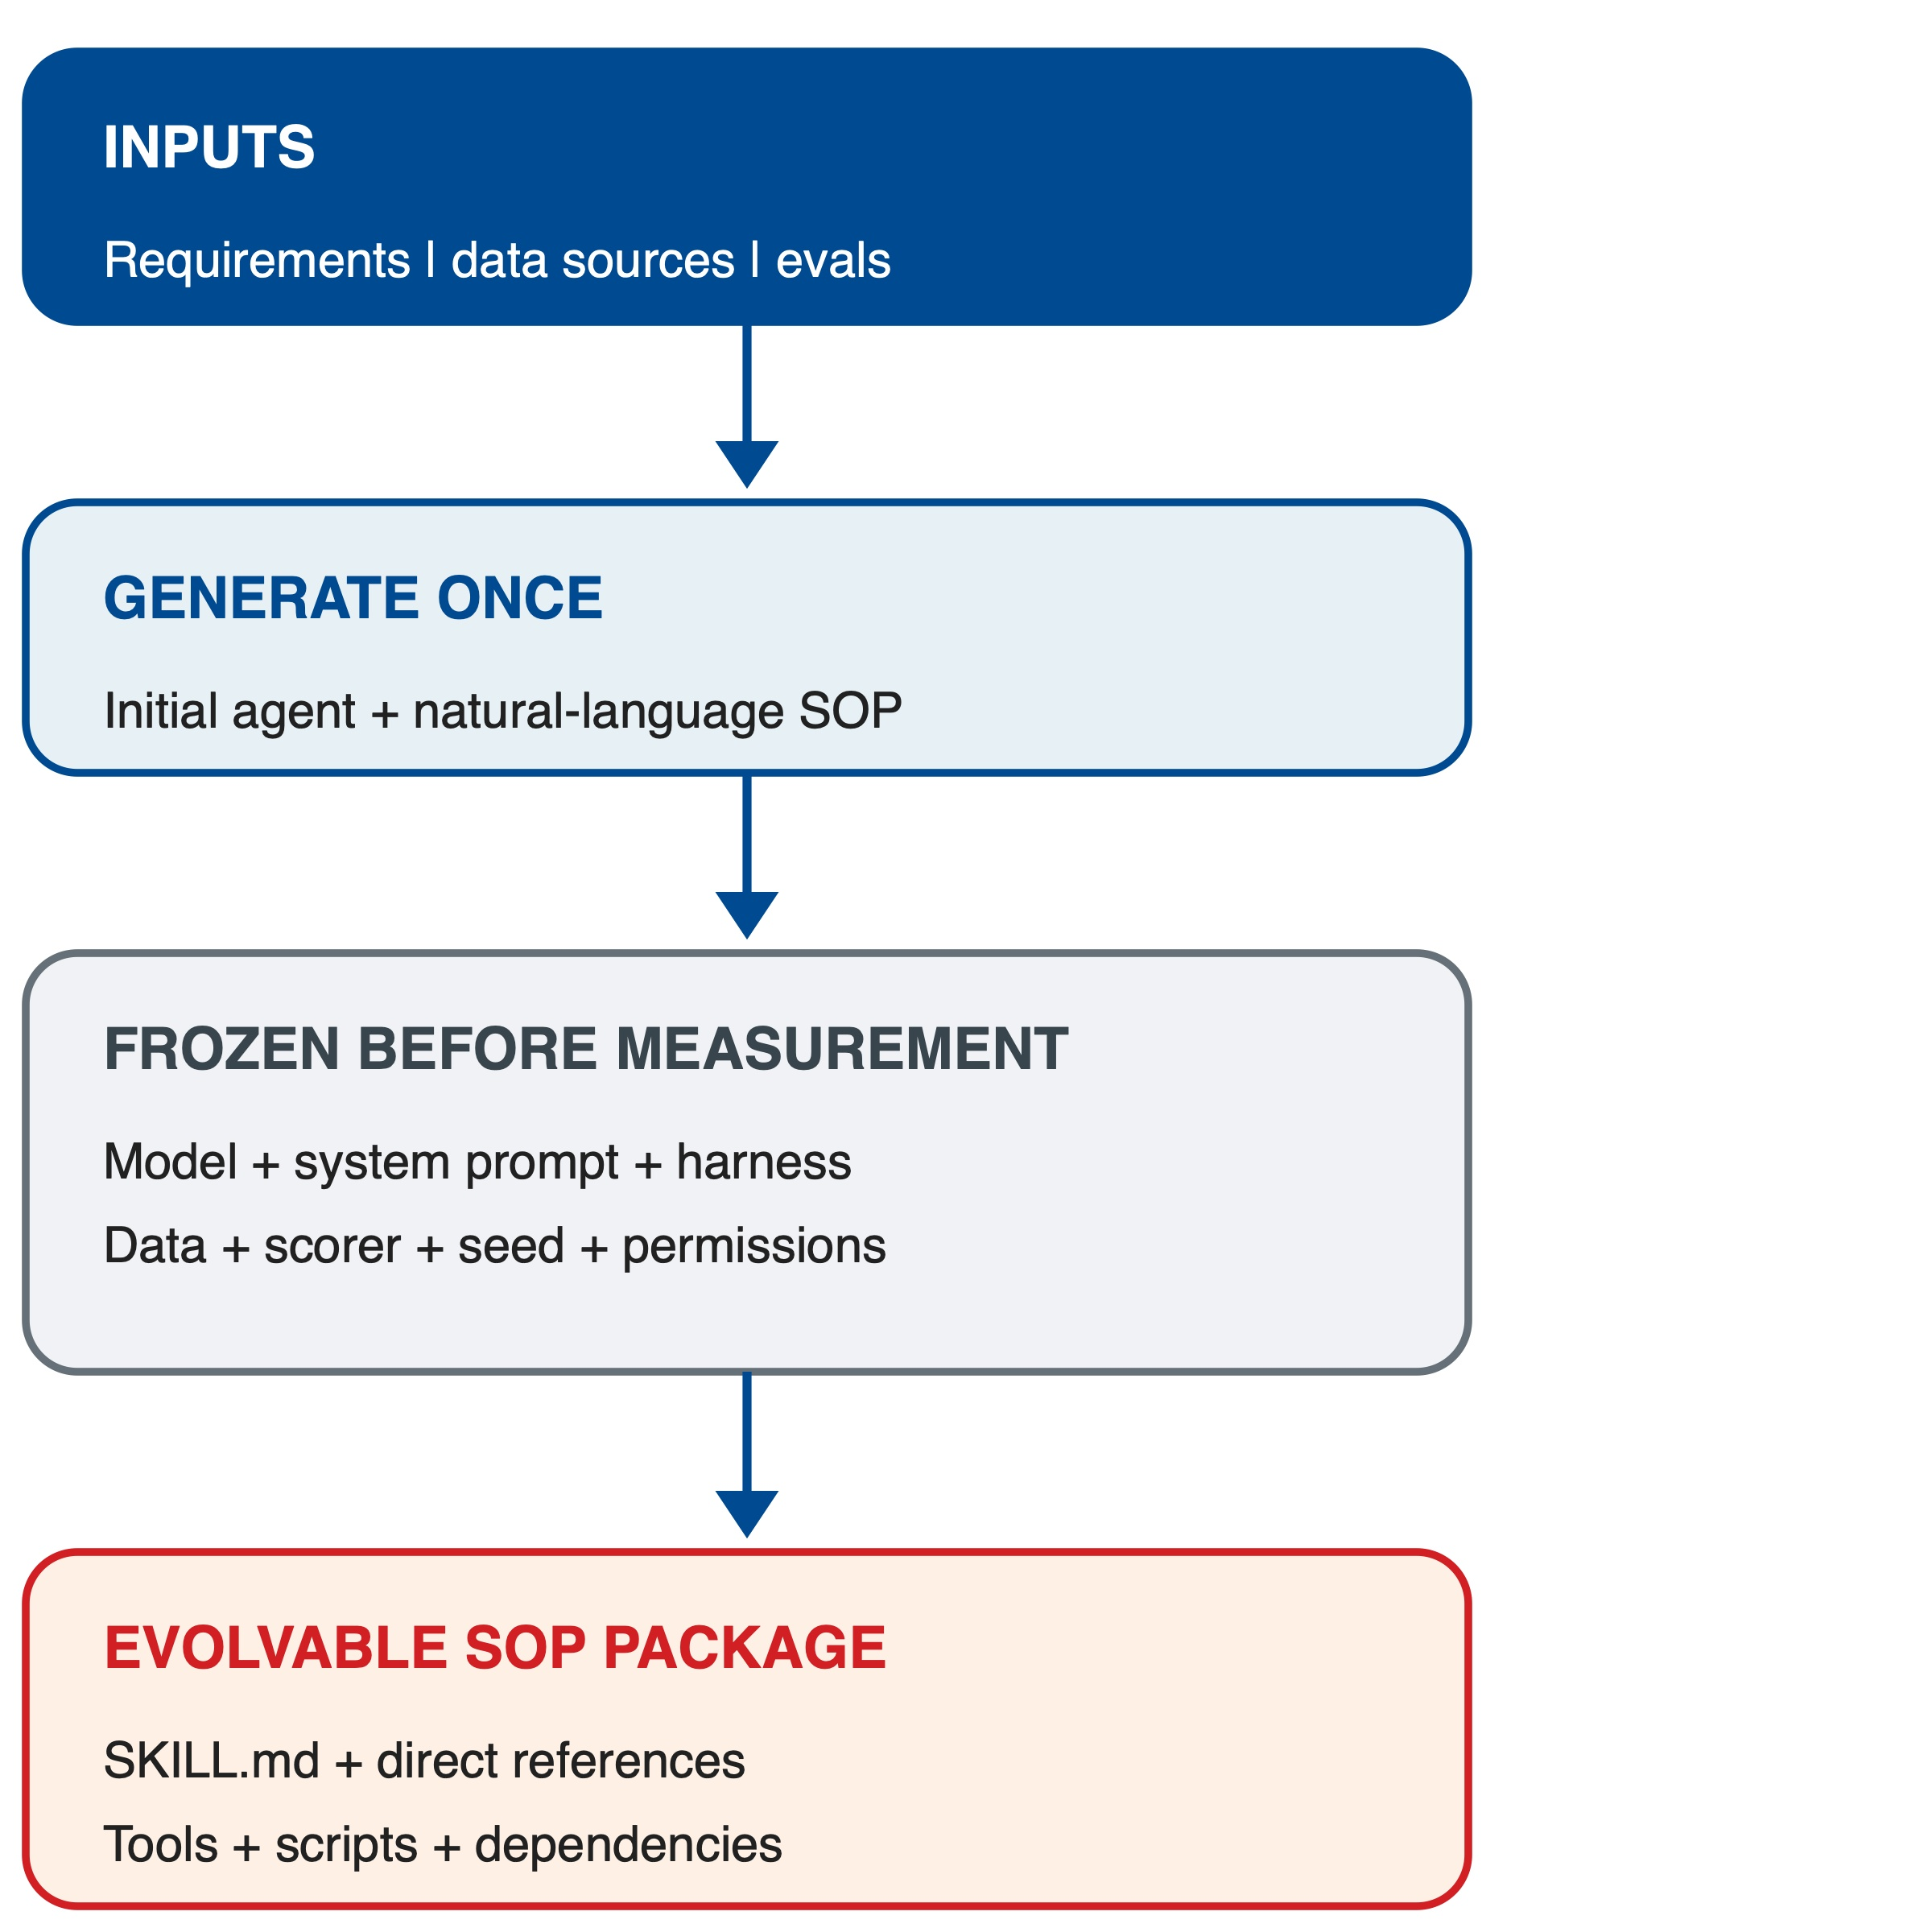
\includegraphics[width=0.64\textwidth]{architecture.jpg}
\caption{Frozen PLaND boundary. The initial agent and evaluation contract are finalized before baseline measurement; only the workflow skill package may evolve.}
\end{figure*}

Every numbered SOP step is marked as an English instruction, a reference to supporting skill material, or a direct Python/Bash command. A command counts as compiled only when the evaluated runtime invokes it and consumes its output. \texttt{SKILL.md} is the SOP source of truth, while the comparison hash also covers directly referenced instructions, invoked scripts, and approved dependencies.

The model and digest, system prompt, normalized harness, evaluation cases and expected outputs, scorer, datasource snapshot, seed, model/runtime settings, permissions, quality floor, non-inferiority margin, and expense objective are frozen. Comparison code rejects mismatched fingerprints, duplicated case identifiers, or missing full hashes. The candidate may change only the skill package. Commands require bounded input/output contracts and an English fallback. Caching and parallelism are allowed only when applied consistently and recorded as runtime invariants.

\begin{figure*}[t]
\centering
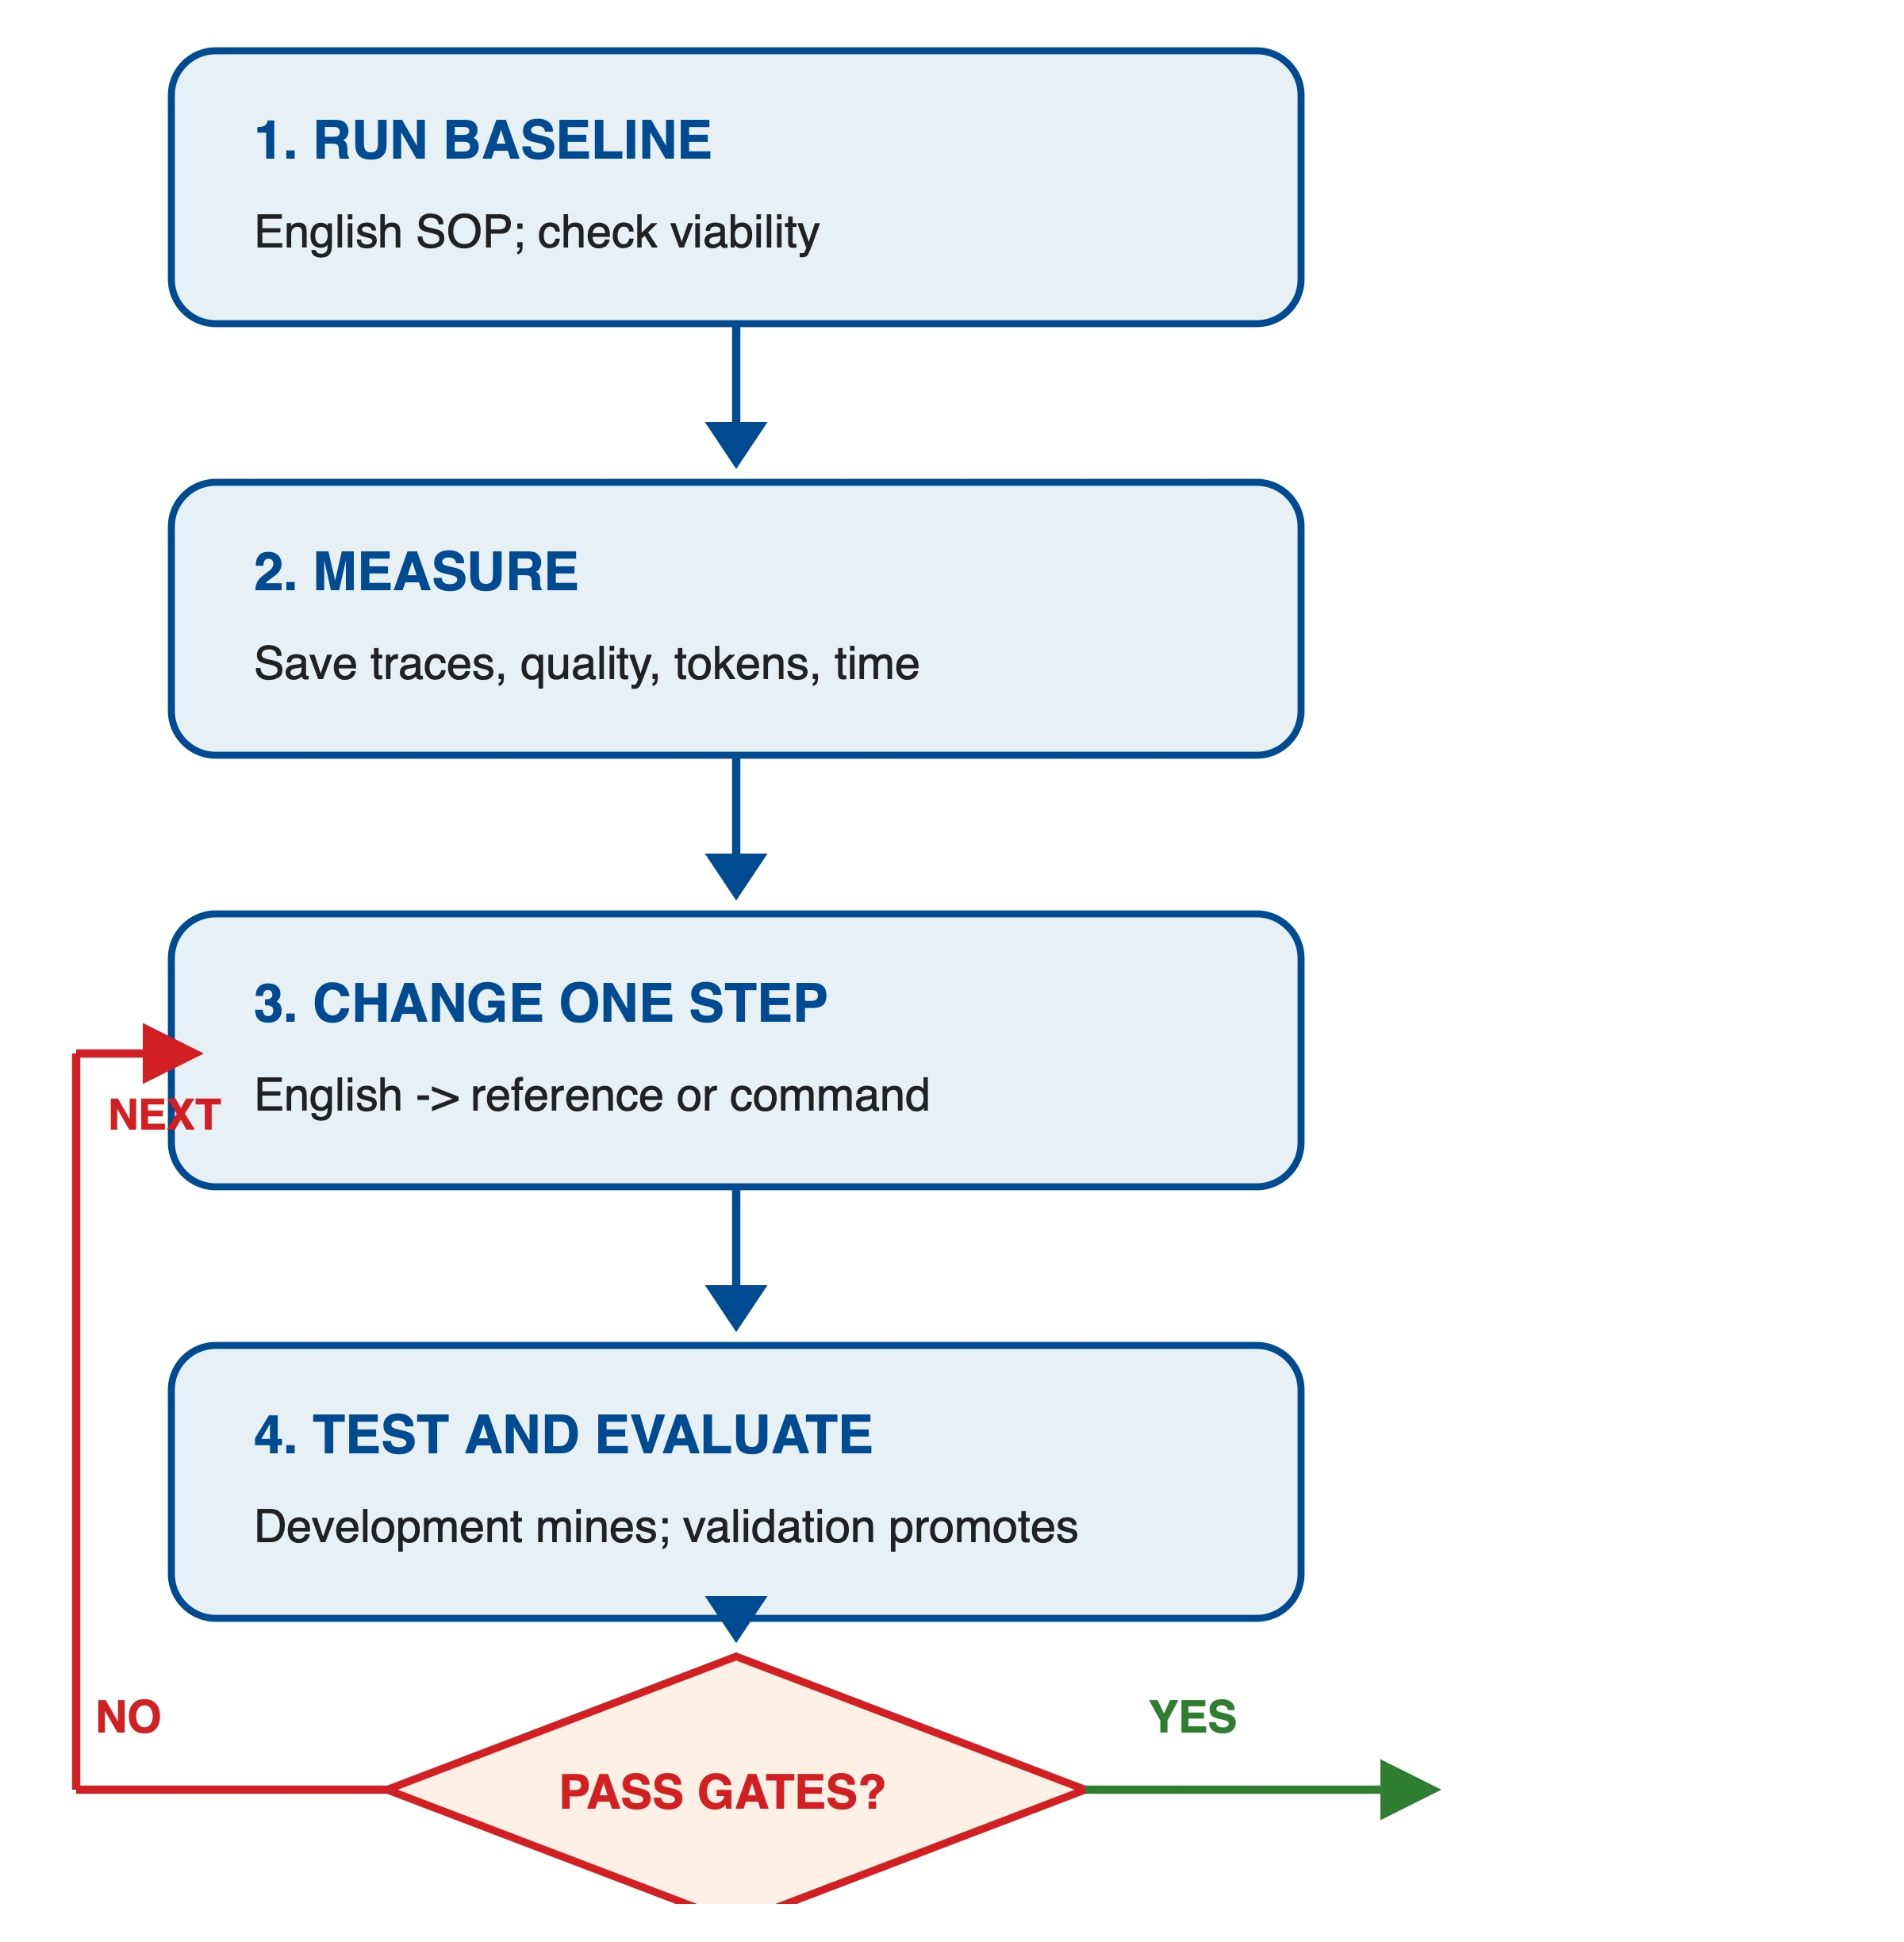
\includegraphics[width=0.62\textwidth]{evolution-loop.jpg}
\caption{One bounded evolution iteration. Development evidence proposes a change; validation promotes it only when frozen quality and expense gates pass.}
\end{figure*}

Evolution was capped at ten candidates. A baseline first had to meet an absolute viability floor. Candidate selection required task quality within a prespecified margin and strict improvement in one primary expense measure. Development informed changes; validation selected candidates; test cases were released once only after validation passed.

\subsection{Data and evaluation}
We prepared public datasets resembling enterprise work: LEDGAR legal clauses [12], CFPB complaint narratives [13], SpamAssassin email [14], SROIE receipts [15], and RVL-CDIP/Tobacco3482 document images [16, 17]. LiteParse supplied a local OCR condition, not a dataset [18]. Selection manifests record source identifiers and hashes, seed 20260902, exclusions, and split membership. Audits checked unique identifiers, split/content overlap, missing files, label leakage, source boundaries, and pilot overlap. The repeated study uses the exact prepared snapshots documented in the \href{https://github.com/mnvsk97/PLaND/tree/codex/pland-variance-study/experiments/ledgar-text-classification/results/variance-study-20260903}{LEDGAR evidence folder}, \href{https://github.com/mnvsk97/PLaND/tree/codex/pland-variance-study/experiments/cfpb-text-classification/results/variance-study-20260903}{CFPB evidence folder}, and \href{https://github.com/mnvsk97/PLaND/tree/codex/pland-variance-study/experiments/spamassassin-email-classification/results/variance-study-20260903}{SpamAssassin evidence folder}.

\begin{table*}[t]
\centering
\small
\caption{Prepared confirmatory datasets}
\begin{tabularx}{\textwidth}{@{}XXX@{}}
\toprule
Workflow & Development / validation / test & Status \\
\midrule
LEDGAR clause classification & 100 / 100 / 1,000 & Test released; three optimized replications \\
CFPB complaint routing & 100 / 100 / 1,000 & Three validation rejections; test not released \\
SpamAssassin email classification & 100 / 100 / 1,000 & Three validation rejections; test not released \\
QS-OCR/Tobacco3482 classification & 100 / 100 / 1,000 & Prepared; baseline nonviable \\
SROIE receipt extraction & 100 / 100 / 300 & Prepared; baseline nonviable \\
RVL-CDIP constrained mirror & 100 / 100 / 369 & Prepared; baseline nonviable \\
\bottomrule
\end{tabularx}
\end{table*}

Classification required both variants to reach 0.80 accuracy. Extraction required field F1 of at least 0.50. For baseline b and hybrid h, the lower bound of a paired bootstrap 95\% interval for \texttt{accuracy\_h - accuracy\_b} had to be at least -0.02. Token reduction had to be at least 5\%, with a positive bootstrap lower bound. We used 5,000 paired resamples with seed 20260902, Wilson accuracy intervals, and an exact McNemar test.

Text experiments used local Ollama 0.33.0 and \texttt{qwen3:14b}, digest \texttt{bdbd181c33f2}\allowbreak\texttt{ed1b31c97299}\allowbreak\texttt{1882db3cf4d1}\allowbreak\texttt{92569092138a}\allowbreak\texttt{7d29e973cd9d}\allowbreak\texttt{ebe8}, on an Apple M5 Pro with 48 GB unified memory. Original confirmatory runs were sequential. The repeated optimized study disabled thinking and streaming; used temperature 0, seeds 20260903-20260905, a 4,096-token context, a 128-token output cap, and an exact JSON schema; preloaded and retained the model; and enabled Flash Attention, q8\_0 KV cache, one loaded model, and two parallel requests. The same seed was used within each NL/hybrid pair. Order was NL-hybrid, hybrid-NL, then NL-hybrid. Checkpoints, exact commands, timestamps, hashes, component durations, per-case latency/tokens/routing, and wall time were stored. The original sequential run is not pooled with these two-worker replications, and every repeated LEDGAR test evaluation is a replication rather than an untouched test.

\section{Results}
\begin{table*}[t]
\centering
\small
\caption{Three-run optimized replication results}
\begin{tabularx}{\textwidth}{@{}XXXX@{}}
\toprule
Workflow and split & Accuracy mean (sample SD), NL -> hybrid & Mean tokens, NL -> hybrid & Decision across runs \\
\midrule
LEDGAR test (1,000) & 93.7\% (0) -> 92.9\% (0) & 376,090 -> 225,575.33 (-40.02\%) & 3/3 pass \\
CFPB validation (100) & 78.0\% (0) -> 71.0\% (0) & 58,372 -> 33,120 (-43.26\%) & 0/3; reject quality/viability \\
SpamAssassin validation (100) & 88.0\% (0) -> 85.0\% (0) & 188,384 -> 178,880.67 (-5.04\%) & 0/3; reject quality \\
\bottomrule
\end{tabularx}
\end{table*}

The original 1,000-case LEDGAR test produced a -0.8-point hybrid-minus-NL accuracy difference (95\% interval [-1.6, 0.0]) and passed the prespecified gate. Each new replication also produced a -0.8-point difference; bootstrap intervals were [-1.6, -0.1], [-1.6, 0.0], and [-1.6, 0.0] points. Each pair had 17 differing predicted labels and passed absolute viability, non-inferiority, and efficiency. The repeated result supports the chosen engineering margin, not equivalence or universal non-inferiority. Exact run and comparison payloads are in the \href{https://github.com/mnvsk97/PLaND/tree/codex/pland-variance-study/experiments/ledgar-text-classification/results/variance-study-20260903}{LEDGAR evidence folder}.

LEDGAR model calls were 1,000 NL and 589 hybrid in every run because the same 411 cases used deterministic commands. NL tokens were exactly 376,090; hybrid tokens ranged from 225,575 to 225,576 (sample SD 0.58). CFPB calls were 100 versus 58 and SpamAssassin calls were 100 versus 97 in every run. Routing never changed across seeds. Each dataset had zero cross-run label disagreement within NL and within hybrid, including separately among stable command-routed and model-fallback cases. This is direct reproducibility evidence under the frozen temperature-zero runtime; because both variants reached the same zero-disagreement floor, it does not show that hybrid execution reduced variance relative to NL.

CFPB repeated the same rejection three times: 43.26\% token savings, 78\% NL versus 71\% hybrid accuracy, paired difference intervals of [-13, -2] points, and failure of the 80\% floor. SpamAssassin repeated 5.04\% savings, 88\% versus 85\% accuracy, and non-inferiority failure in all three runs. Neither test set was released; exact comparisons are in the \href{https://github.com/mnvsk97/PLaND/tree/codex/pland-variance-study/experiments/cfpb-text-classification/results/variance-study-20260903}{CFPB} and \href{https://github.com/mnvsk97/PLaND/tree/codex/pland-variance-study/experiments/spamassassin-email-classification/results/variance-study-20260903}{SpamAssassin} evidence folders. QS-OCR/Tobacco3482 remains a single-baseline classification feasibility failure at 70\% accuracy. SROIE remains a separate single-baseline extraction failure at 0.344 field F1 with OCR word-error rate 0.676. RVL-CDIP remains a single-baseline classification feasibility failure at 50\% accuracy. Accuracy, field F1, and OCR error are not combined.

\section{Discussion}
The main result is not that hybrid workflows always win. It is that PLaND exposes when deterministic substitution is acceptable. LEDGAR retained accuracy within a prespecified engineering margin while eliminating 41.1\% of model calls. The mechanism decomposition is important: prompt compression explained only 2.76\% of savings, whereas call bypass explained 97.24\%. CFPB and SpamAssassin show that lower token use alone is insufficient.

The methodology supports an evidence-driven progression. An unfamiliar task may remain an open-ended agent. Stable steps can move into commands while semantic judgment remains in language. A mature workflow may become a graph, but conversion stops whenever quality declines. References help manage large instructions; they are not automatically deterministic. Runtime guards, fallback, canary monitoring, and automatic demotion are specified design extensions but were not used to obtain these results.

Several assumptions bound interpretation. Dataset labels and selected samples are treated as the evaluation target; the balanced LEDGAR subset does not estimate full multi-label or production prevalence. Tokens and model calls are expense proxies, not measured currency, energy, or carbon. The text experiments test harness-level routing, not autonomous DeepAgent command interpretation. The 2-point margin and 80\% floor are task-design choices rather than universal standards. Only three seeds, one local model, one machine, and one temperature-zero runtime were studied. Zero observed disagreement is descriptive, may reflect the deterministic runtime floor, and is not evidence of significance or broad stochastic robustness. Parallel timing can vary with warm-up, caching, scheduling, and thermal state and cannot be compared causally with the sequential study. SROIE and RVL test sizes were constrained by eligible source data. Author-designed rules may not transfer to other domains, and the generalized generator/evolver was not reevaluated end to end here.

Future work should repeat paired conditions across models and less deterministic sampling regimes, add tool-sequence disagreement, test natural-language and no-skill ablations, and evaluate runtime fallback and demotion. Stateful environments such as tau-bench remain future work and should use final-state and action verification rather than classification accuracy; PLaND leaves that scorer task-defined.

\section{Conclusion}
PLaND is a methodology for selectively moving stable agent work from natural language into tested code under a frozen evaluation contract. Across three optimized LEDGAR replications, the accepted hybrid passed every gate, reduced mean tokens by 40.02\%, and replaced 411 model calls with commands. CFPB and SpamAssassin repeated their rejection outcomes, while three image workflows remain distinct single-baseline feasibility failures. Both text variants showed zero cross-run label disagreement, so the evidence supports reproducibility in this frozen condition but not hybrid-specific variance reduction. The practical rule is simple: keep judgment where it adds value, compile stable operations where evidence permits, and preserve rejection evidence when it does not.

\section{Acknowledgements}
None.

\section{Disclosure and Conflict of Interest}
This work received no external funding. The authors declare no conflicts of interest.

\section{Data and Code Availability}
Source code, methodology skills, preparation scripts, exact commands, logs, per-case safe traces, comparisons, and SHA-256 manifests are preserved in the same Git commit as this manuscript, on branch \texttt{codex/pland-variance-study} at \url{https://github.com/mnvsk97/PLaND/tree/codex/pland-variance-study} The repeated results are in the exact \href{https://github.com/mnvsk97/PLaND/tree/codex/pland-variance-study/experiments/ledgar-text-classification/results/variance-study-20260903}{LEDGAR}, \href{https://github.com/mnvsk97/PLaND/tree/codex/pland-variance-study/experiments/cfpb-text-classification/results/variance-study-20260903}{CFPB}, and \href{https://github.com/mnvsk97/PLaND/tree/codex/pland-variance-study/experiments/spamassassin-email-classification/results/variance-study-20260903}{SpamAssassin} folders. Large copyrighted or sensitive source records are not redistributed; the repository records their sources, selection procedures, and hashes for authorized reproduction. An arXiv-ready bundle is prepared locally but has not been submitted, so the arXiv identifier remains pending.

\begin{thebibliography}{99}
\bibitem{ref1} Agent Skills. (2026). \emph{Agent Skills specification}. \url{https://agentskills.io/specification}
\bibitem{ref2} LangChain. (2026). \emph{DeepAgents: Skills}. \url{https://docs.langchain.com/oss/python/deepagents/skills}
\bibitem{ref3} LangChain. (2026). \emph{LangGraph overview}. \url{https://docs.langchain.com/oss/python/langgraph/overview}
\bibitem{ref4} Khattab, O., et al. (2023). DSPy: Compiling declarative language model calls into self-improving pipelines. \emph{arXiv}. \url{https://arxiv.org/abs/2310.03714}
\bibitem{ref5} Li, Z., et al. (2024). AutoFlow: Automated workflow generation for large language model agents. \emph{arXiv}. \url{https://arxiv.org/abs/2407.12821}
\bibitem{ref6} Zhang, J., et al. (2024). AFlow: Automating agentic workflow generation. \emph{arXiv}. \url{https://arxiv.org/abs/2410.10762}
\bibitem{ref7} Hu, S., Lu, C., \& Clune, J. (2024). Automated design of agentic systems. \emph{NeurIPS}. \url{https://arxiv.org/abs/2408.08435}
\bibitem{ref8} Yang, Y., et al. (2026). SkillOpt: Executive strategy for self-evolving agent skills. \emph{arXiv}. \url{https://arxiv.org/abs/2605.23904}
\bibitem{ref9} Liu, Y., et al. (2026). SkillRevise: Improving LLM-authored agent skills via trace-conditioned skill revision. \emph{arXiv}. \url{https://arxiv.org/abs/2606.01139}
\bibitem{ref10} Gao, Y., et al. (2026). SkillReducer: Optimizing LLM agent skills for token efficiency. \emph{arXiv}. \url{https://arxiv.org/abs/2603.29919}
\bibitem{ref11} Kevin, C., et al. (2026). Evaluating skills, not just agents: Agentic continuous evaluation of skills. \emph{arXiv}. \url{https://arxiv.org/abs/2608.20614}
\bibitem{ref12} Tuggener, D., et al. (2020). LEDGAR: A large-scale multi-label corpus for text classification of legal provisions in contracts. \emph{LREC 2020}, 1235-1241. \url{https://aclanthology.org/2020.lrec-1.155/}
\bibitem{ref13} Consumer Financial Protection Bureau. (2026). \emph{Consumer Complaint Database}. \url{https://www.consumerfinance.gov/data-research/consumer-complaints/}
\bibitem{ref14} Apache SpamAssassin. (2006). \emph{Public corpus}. \url{https://spamassassin.apache.org/old/publiccorpus/}
\bibitem{ref15} Huang, Z., et al. (2021). ICDAR2019 competition on scanned receipt OCR and information extraction. \emph{arXiv}. \url{https://arxiv.org/abs/2103.10213}
\bibitem{ref16} Harley, A. W., Ufkes, A., \& Derpanis, K. G. (2015). Evaluation of deep convolutional nets for document image classification and retrieval. \emph{ICDAR 2015}. \url{https://arxiv.org/abs/1502.07058}
\bibitem{ref17} Lim, G., Larson, S., \& Leach, K. (2024). Label errors in the Tobacco3482 dataset. \emph{arXiv}. \url{https://arxiv.org/abs/2412.13140}
\bibitem{ref18} LlamaIndex. (2026). \emph{LiteParse: Open-source document parsing}. \url{https://github.com/run-llama/liteparse}
\end{thebibliography}
\end{document}
